\documentclass[11pt,a4paper]{article}

\usepackage[margin=1in]{geometry}
\usepackage[T1]{fontenc}
\usepackage[utf8]{inputenc}
\usepackage{lmodern}
\usepackage{amsmath,amssymb}
\usepackage{booktabs}
\usepackage{array}
\usepackage{graphicx}
\usepackage{adjustbox}
\usepackage{caption}
\usepackage{subcaption}
\usepackage{float}
\usepackage[table]{xcolor}
\usepackage{hyperref}
\usepackage{enumitem}
\setlength{\emergencystretch}{3em}

\hypersetup{
    colorlinks=true,
    linkcolor=blue,
    citecolor=blue,
    urlcolor=blue
}

\graphicspath{{../docs/slides/HUST_THEME_BEAMER/photos/}{../docs/slides/HUST_THEME_BEAMER/images/}}

\newcommand{\method}{\texorpdfstring{$M^2$-CL}{M2-CL}}
\newcommand{\base}{\texorpdfstring{$M^2$}{M2}}
\newcommand{\codepath}[1]{\texttt{#1}}
\definecolor{headerblue}{HTML}{E7F0FA}
\definecolor{lightgreen}{HTML}{EAF7EA}
\definecolor{lightyellow}{HTML}{FFF6D8}
\definecolor{lightred}{HTML}{FDEAEA}
\newcommand{\pos}[1]{\textcolor{green!45!black}{+#1}}

\title{\textbf{Multiscale and Multilayer Contrastive Learning for Domain Generalization}\\
\large Course Project Report}
\author{
Group 26\\
Vu Thuong Tin \quad Chu Anh Duc \quad Nguyen Xuan Khai
}
\date{\today}

\begin{document}
\pagenumbering{Alph}
\begin{titlepage}
    \thispagestyle{empty}
    \centering
    \vspace*{1.2cm}
    {\Large Hanoi University of Science and Technology\par}
    \vspace{0.4cm}
    {\large School of Information and Communication Technology\par}
    \vspace{1.8cm}
    {\Huge\bfseries Course Project Report\par}
    \vspace{0.7cm}
    {\LARGE Multiscale and Multilayer Contrastive Learning\\for Domain Generalization\par}
    \vspace{0.8cm}
    {\Large Reproduction, Implementation Analysis, and Experimental Discussion\par}
    \vfill
    \begin{tabular}{rl}
        \textbf{Group:} & 26\\
        \textbf{Students:} & Vu Thuong Tin\\
                         & Chu Anh Duc\\
                         & Nguyen Xuan Khai\\
        \textbf{Project topic:} & Domain Generalization in Computer Vision\\
        \textbf{Main method:} & \method{}\\
    \end{tabular}
    \vfill
    {\large \today\par}
\end{titlepage}

\pagenumbering{roman}
\tableofcontents
\newpage
\pagenumbering{arabic}

\begin{abstract}
Domain generalization (DG) studies the problem of training a visual recognition model on a set of source domains and deploying it on unseen target domains without access to target-domain samples during training. This setting is difficult because convolutional neural networks often exploit domain-specific shortcuts such as background, texture, rendering style, or acquisition bias instead of learning class-causal visual attributes. This report presents a course-project reproduction and analysis of \method, a multiscale and multilayer contrastive learning framework for DG. Unlike the original research paper, this document is written as a university project report: it explains the motivation, connects the mathematical idea to the implementation in the submitted codebase, describes the training pipeline, discusses the experimental results, and reflects on practical reproducibility issues. The method extends a standard ImageNet-pretrained ResNet backbone with extraction blocks attached to intermediate convolutional layers. These blocks compress and pool multiscale feature maps into a representation that combines low-level and high-level evidence. A supervised contrastive regularizer is then applied to intermediate representations so that samples of the same class become closer while samples of different classes become more separable. We evaluate the method on PACS, VLCS, and Office-Home using leave-one-domain-out evaluation, compare it against representative DG baselines, and analyze both quantitative accuracy and qualitative saliency-map behavior.
\end{abstract}

\section{Introduction}

Modern image classifiers achieve strong in-distribution performance, but their accuracy can drop sharply when the test images come from a visual context that was absent during training. This is common in practical applications: a model trained on photos may be evaluated on sketches, artworks, cartoons, medical images from another device, or objects captured in a different environment. The central problem is that empirical risk minimization (ERM) does not distinguish between class-causal evidence and domain-specific shortcuts. If a training domain repeatedly associates a class with a background, texture, or color distribution, a high-capacity CNN can learn that correlation and still achieve low source-domain error.

Domain generalization addresses this failure mode under a strict constraint: target-domain images and labels are unavailable during training. A DG model must therefore learn representations that remain useful under distribution shift by relying only on the diversity present in source domains. The paper \textit{Multiscale and Multilayer Contrastive Learning for Domain Generalization} by Ballas and Diou proposes that intermediate CNN features contain useful information for separating invariant class attributes from domain-specific artifacts. Instead of using only the last feature vector of a ResNet, the method extracts representations from multiple layers and multiple spatial scales.

This project implements and analyzes the core idea of that paper. The presentation slides focus on three standard DG benchmarks used in the original work: PACS, VLCS, and Office-Home.

\subsection{Project Motivation}

The motivation of this project is not only to restate the paper but also to understand whether the method can be reconstructed as a working training pipeline. This distinction matters in a course project. A research paper normally emphasizes novelty, mathematical formulation, and final benchmark numbers. A project report should additionally answer more practical questions:

\begin{itemize}[leftmargin=1.4em]
    \item What exact problem is being solved, and why is the usual supervised-learning setting insufficient?
    \item Which part of the published method is implemented in code, and which parts are simplified or left out?
    \item How are datasets, domains, training splits, checkpoints, and evaluation metrics organized?
    \item Do the results support the intended conclusion, and where are the uncertainties?
    \item What did the implementation reveal that is not obvious from the paper alone?
\end{itemize}

For that reason, this report treats \method{} as both a computer-vision method and a reproducibility exercise. The method is studied from three angles: the conceptual DG problem, the architecture and loss design, and the concrete PyTorch implementation in the submitted repository.

\subsection{Report Scope}

The current repository focuses on PACS, VLCS, and Office-Home because those are the datasets used in the project tables and slides.

The implementation supports more methods than are deeply analyzed in the main text. The comparison tables include ERM, RSC, CORAL, Mixup, MMD, SagNet, SelfReg, ARM, EQRM, SAGM, \base{}, and \method{}. However, the main technical discussion focuses on the difference between ERM, \base{}, and \method{}, because these three models isolate the two core ideas of the project: multilayer feature extraction and contrastive regularization.

\subsection{Main Contributions of This Report}

This project report makes the following contributions relative to the original paper:

\begin{enumerate}[leftmargin=1.6em]
    \item It explains the paper's DG setting in a course-report style, with explicit source-domain and target-domain notation.
    \item It maps the proposed architecture to the local model, extraction-block, loss, and training modules.
    \item It summarizes the implemented training and evaluation workflow, including dataset construction, source validation holdout, checkpoint selection, and result aggregation.
    \item It summarizes the experimental workflow and result tables in a form suitable for project defense and written submission.
    \item It adds practical observations about memory usage, batch composition, and reproducibility that are important when turning a paper into code.
\end{enumerate}

\section{Problem Formulation}

Let $\mathcal{D} = \{D_1, D_2, \ldots, D_N\}$ be a set of source domains. Each domain contains image-label pairs $(x,y)$ sampled from a domain-specific joint distribution over $\mathcal{X} \times \mathcal{Y}$. In the leave-one-domain-out protocol, one domain is selected as the unseen target domain, while the remaining domains are used for training and validation. The goal is to learn a classifier
\[
    f_\theta: \mathcal{X} \rightarrow \mathcal{Y}
\]
that minimizes target-domain error despite never observing target-domain data during training.

The key challenge is representation entanglement. A latent representation may contain both class-specific attributes, such as object shape and discriminative parts, and domain-specific attributes, such as sketch strokes, cartoon color palettes, background scenes, lighting, or image texture. If the classifier relies heavily on the latter, it may fail when the target domain changes. The desired behavior is therefore to produce features that preserve class information while suppressing unstable domain-specific correlations.

\section{Related Work}

Several families of methods have been proposed for DG. ERM is the simplest baseline and trains a classifier by minimizing cross-entropy over pooled source-domain data. Regularization methods such as RSC suppress dominant features during training to prevent the model from relying on narrow shortcuts. Distribution alignment methods such as CORAL and MMD encourage feature distributions from different domains to become closer. Data-mixing methods such as Mixup construct interpolated training samples to improve smoothness and robustness. Style-oriented methods such as SagNet attempt to reduce dependence on domain-specific style. Other methods, including ARM, EQRM, SelfReg, and SAGM, introduce meta-learning, risk distribution, self-supervised regularization, or sharpness-aware training mechanisms.

\method{} differs from these approaches by explicitly reusing intermediate convolutional features and regularizing them with a supervised contrastive objective. This design is motivated by the idea that early and middle CNN layers can still contain spatial and local visual evidence that may be lost or entangled by the final global representation.

\begin{table}[H]
\centering
\caption{High-level comparison of DG method families used in the project.}
\label{tab:method_families}
\small
\begin{adjustbox}{max width=\textwidth}
\begin{tabular}{lll}
\toprule
Family & Representative methods & Main idea \\
\midrule
Standard supervision & ERM & Pool all source domains and minimize cross-entropy. \\
Feature suppression & RSC & Hide highly predictive features to reduce shortcut reliance. \\
Distribution alignment & CORAL, MMD & Penalize differences between source-domain feature distributions. \\
Data interpolation & Mixup & Train on convex combinations of samples and labels. \\
Style robustness & SagNet & Reduce dependence on style-related information. \\
Self/extra regularization & SelfReg, SAGM & Add auxiliary constraints for smoother or more stable features. \\
Risk-based methods & ARM, EQRM & Modify the risk objective to improve robustness across environments. \\
Multilayer extraction & \base{}, \method{} & Use intermediate CNN features and contrastive class alignment. \\
\bottomrule
\end{tabular}
\end{adjustbox}
\end{table}

The table highlights why \method{} is a useful project topic. It is not simply another optimizer or augmentation method. It modifies the representation consumed by the classifier and therefore requires changes in model architecture, loss computation, memory usage, and training-time feature handling.

\section{Proposed Method}

\subsection{Backbone Architecture}

The method uses ImageNet-pretrained ResNet-18 and ResNet-50 backbones. A standard ResNet classifier usually passes the final convolutional output through global pooling and a linear classifier. In contrast, \base{} attaches extraction blocks to selected intermediate layers. These blocks collect feature maps at several depths, compress them, process them at multiple spatial scales, and concatenate the resulting vectors into a hypercolumn-like representation.

\begin{figure}[H]
    \centering
    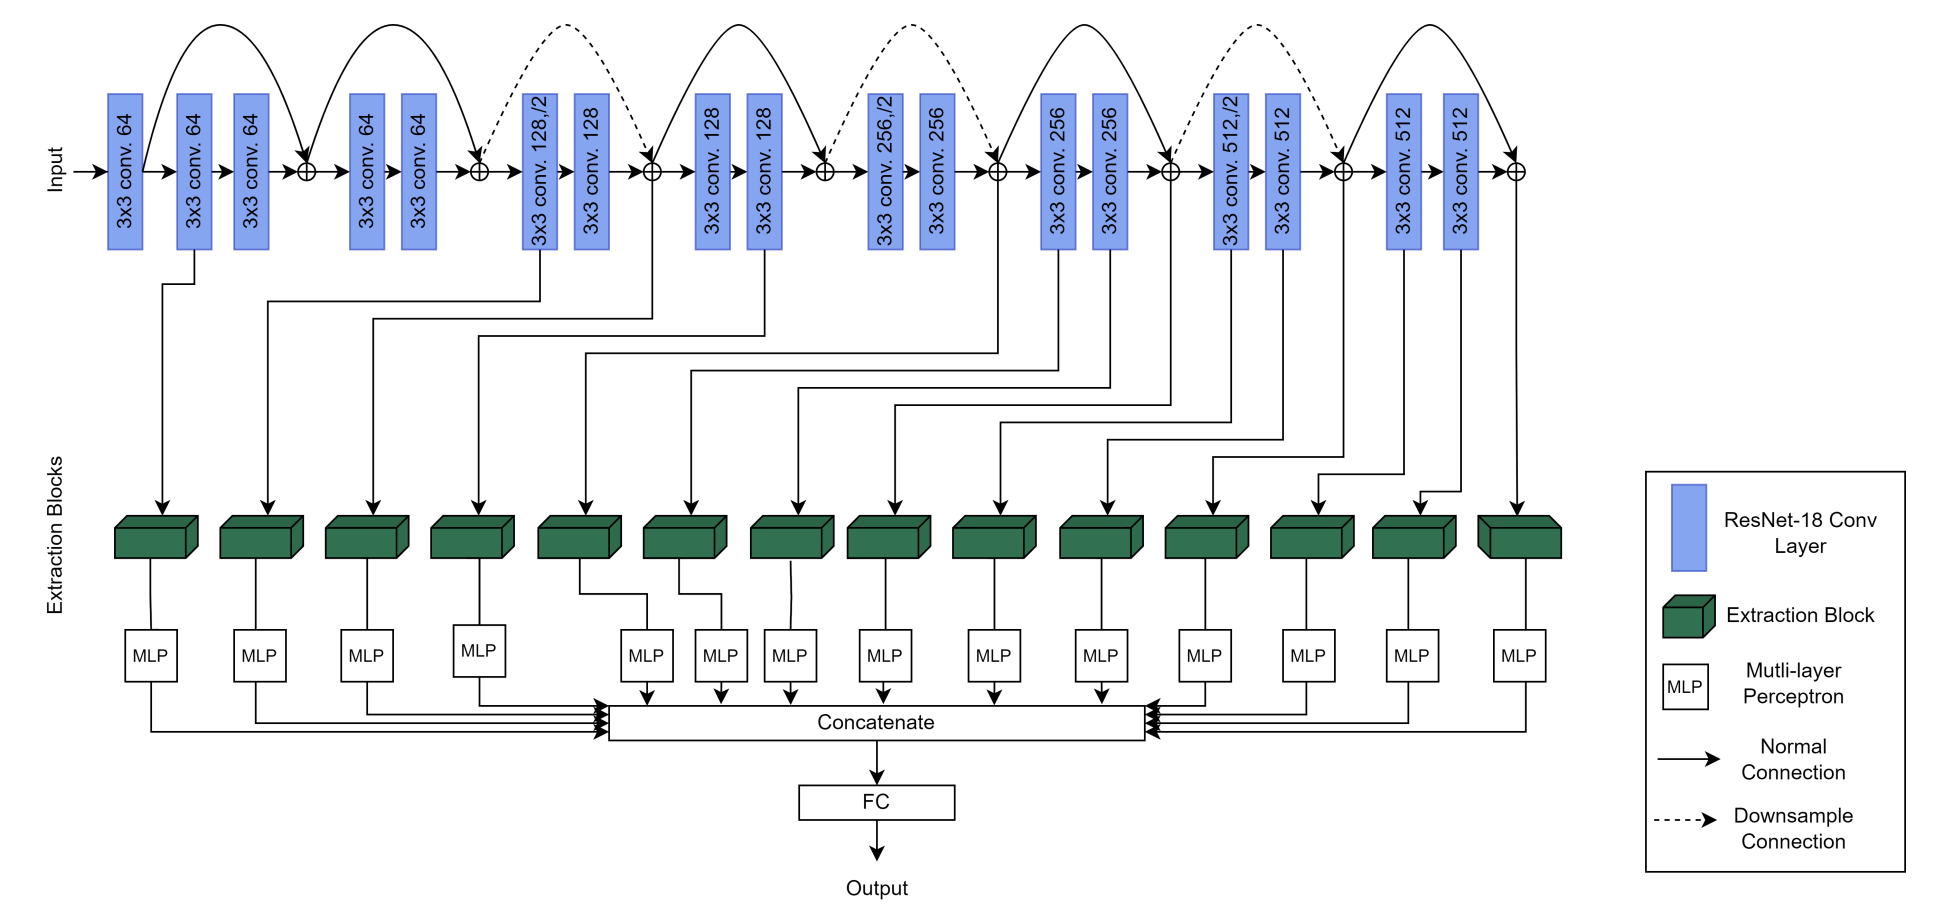
\includegraphics[width=0.82\textwidth]{M2.png}
    \caption{High-level architecture used in the project slides. Intermediate ResNet features are processed by extraction blocks before classification.}
    \label{fig:m2_architecture}
\end{figure}

\begin{figure}[H]
    \centering
    \begin{subfigure}{0.32\textwidth}
        \centering
        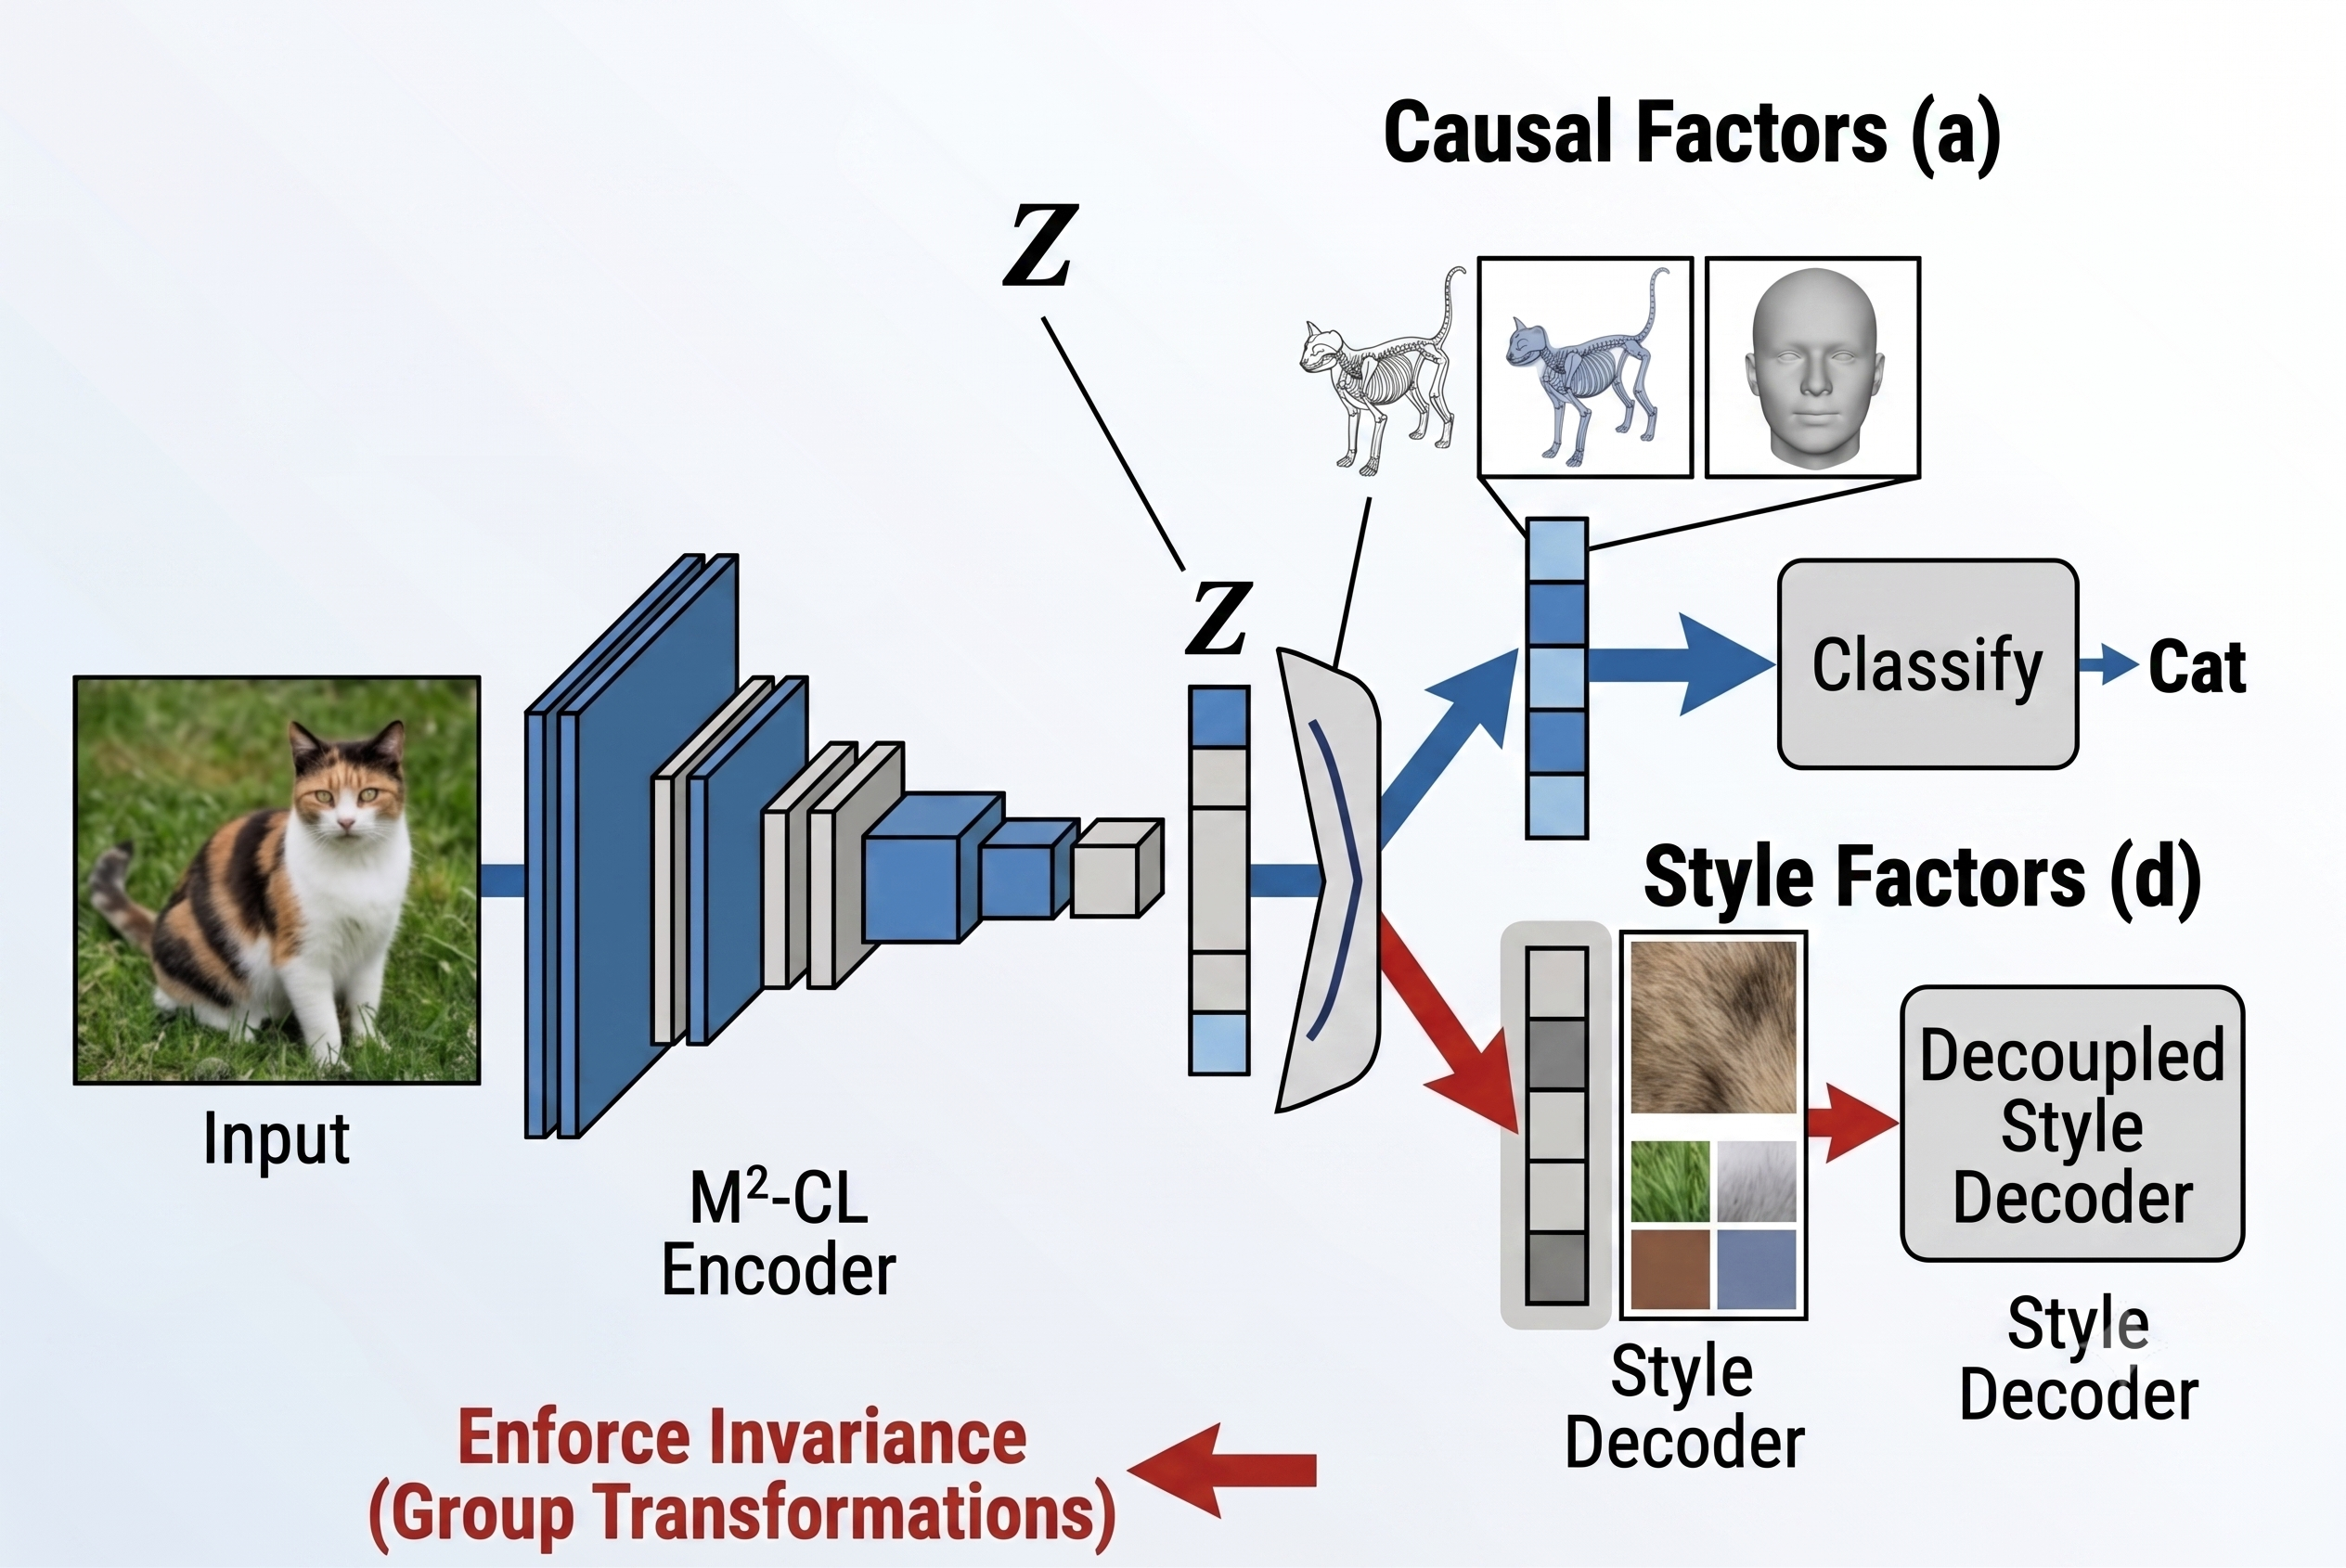
\includegraphics[width=\linewidth]{disentangled.png}
        \caption{Class/domain disentanglement.}
    \end{subfigure}
    \hfill
    \begin{subfigure}{0.32\textwidth}
        \centering
        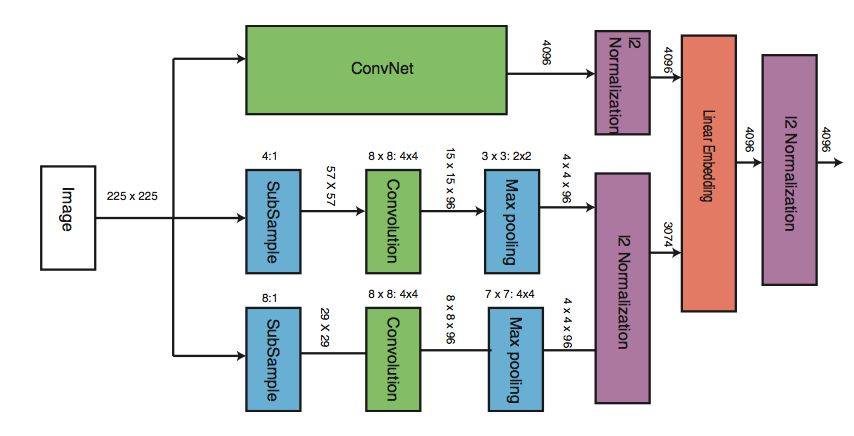
\includegraphics[width=\linewidth]{multilscale.png}
        \caption{Multi-scale evidence.}
    \end{subfigure}
    \hfill
    \begin{subfigure}{0.32\textwidth}
        \centering
        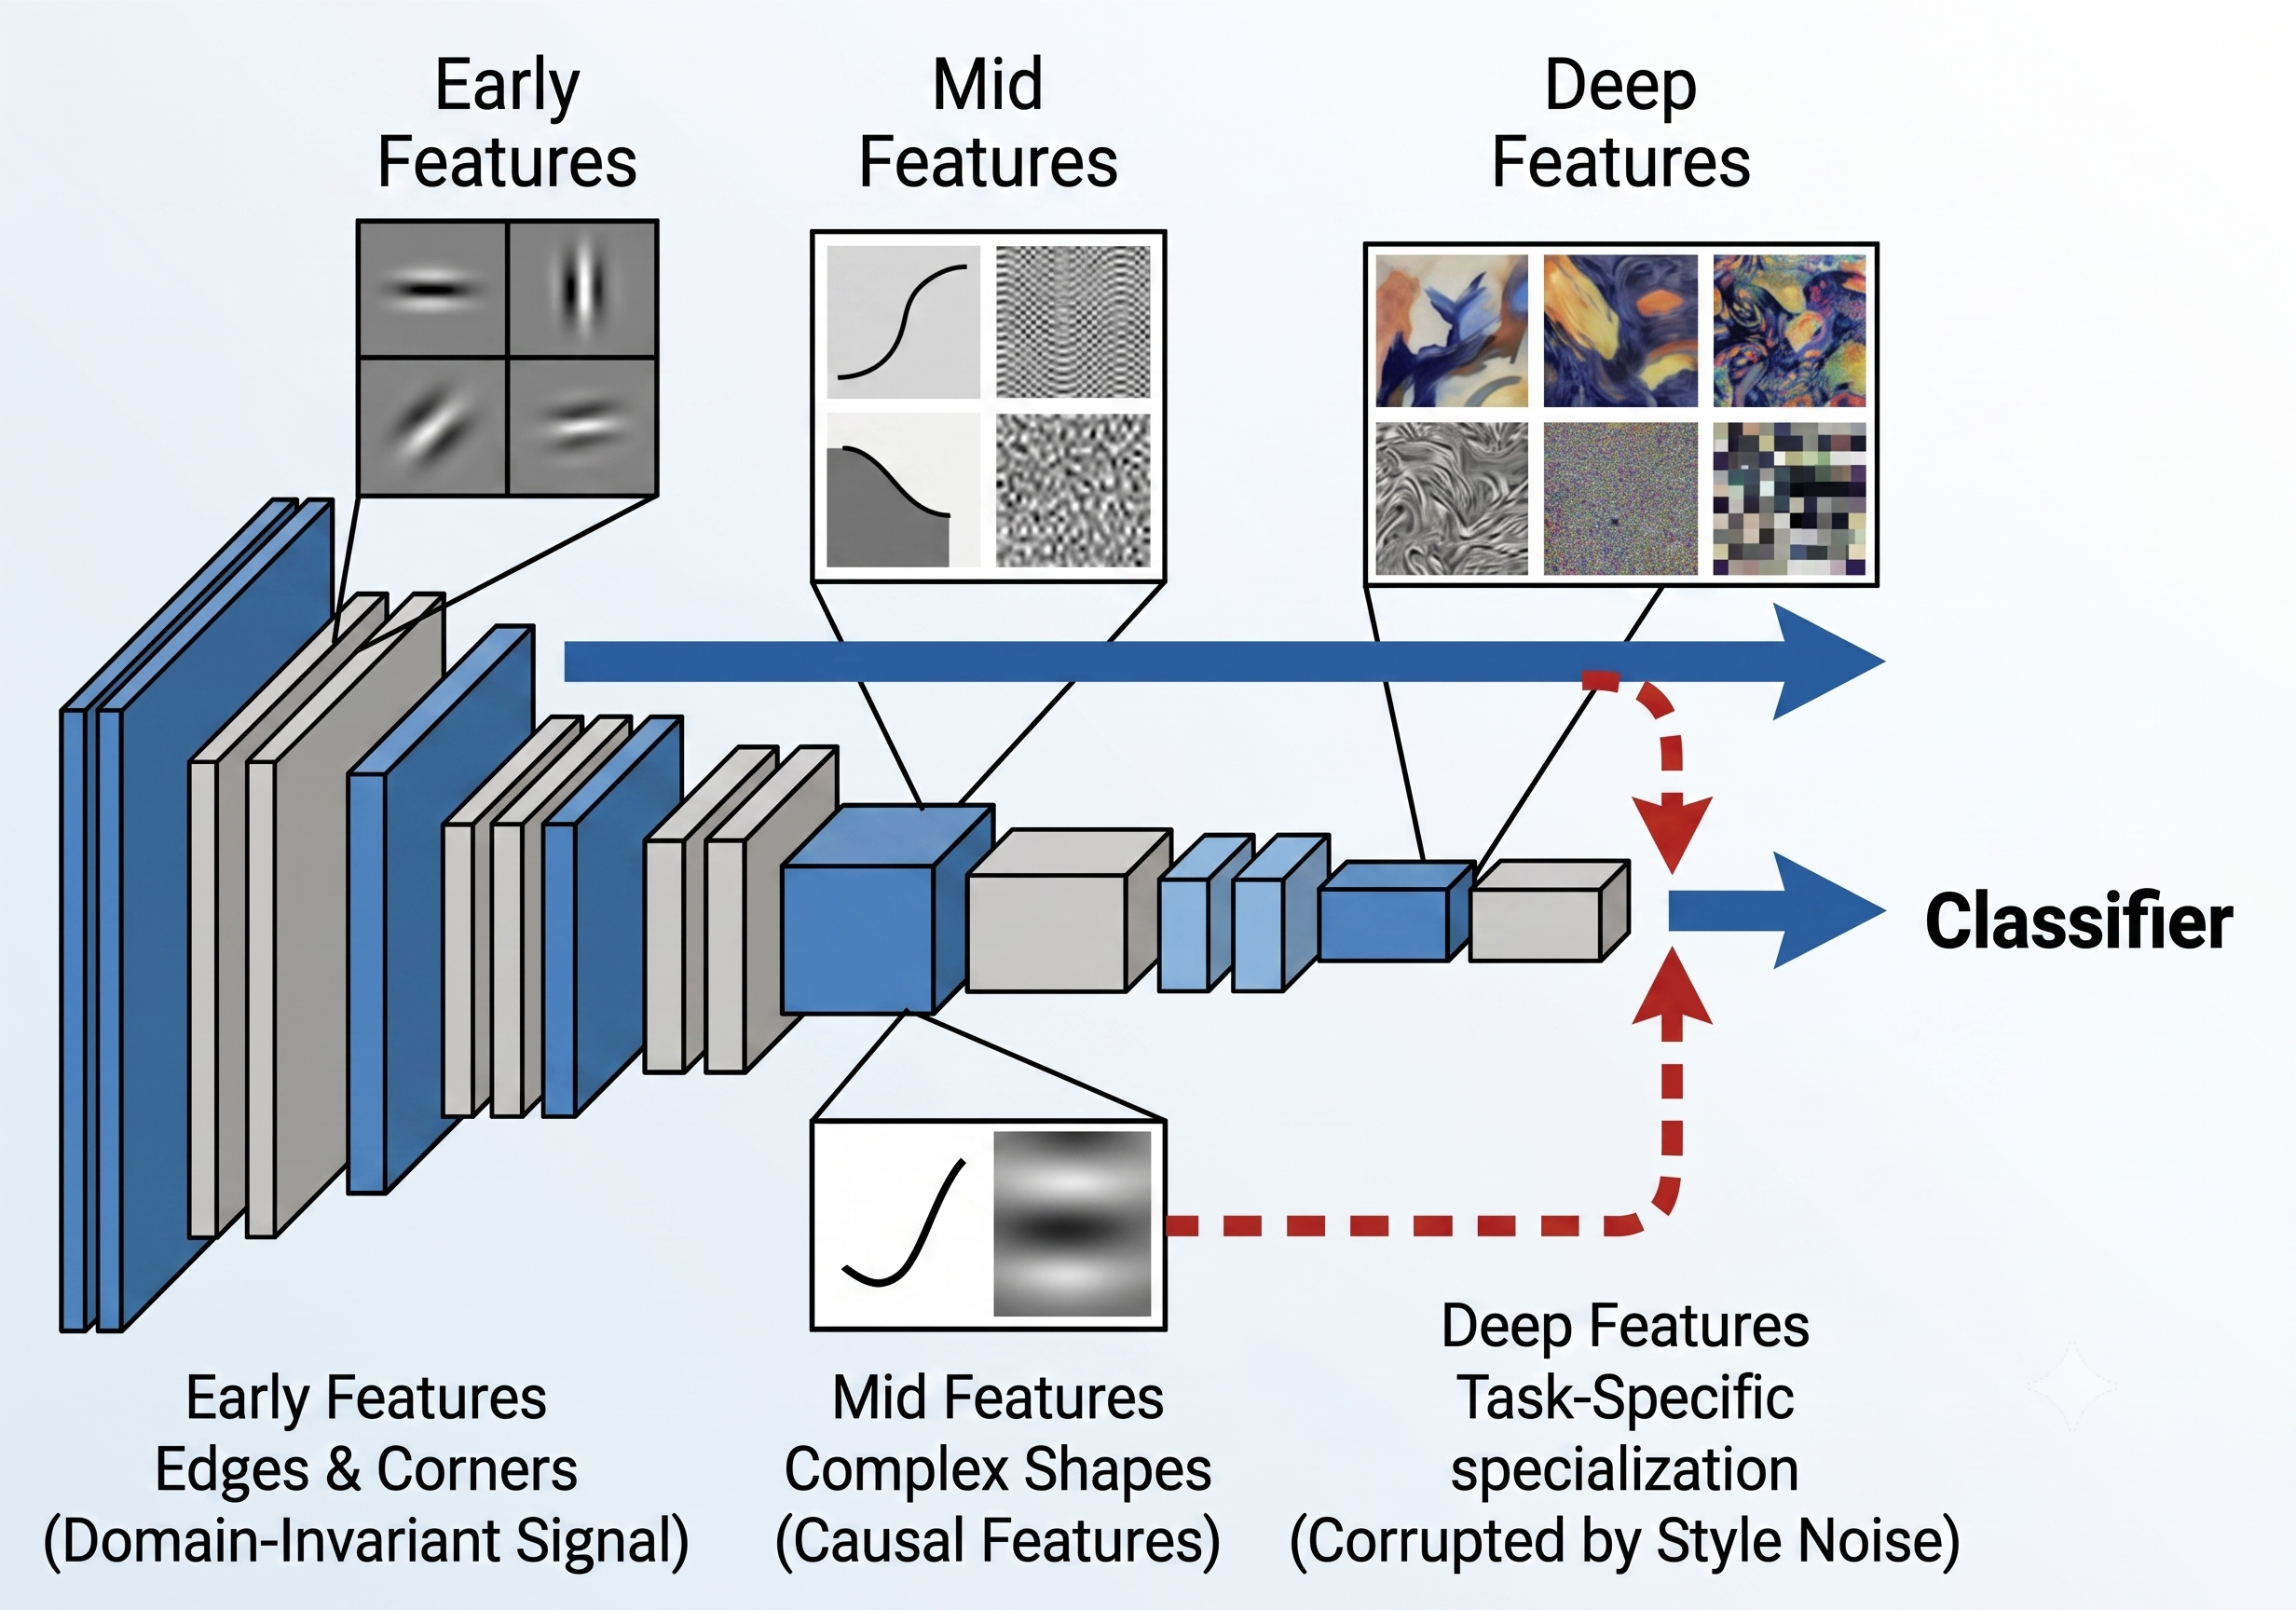
\includegraphics[width=\linewidth]{bottleneck.png}
        \caption{Compressed feature bottleneck.}
    \end{subfigure}
    \caption{Visual intuition behind the method: separate class-relevant and domain-specific attributes, collect information at several spatial scales, and compress intermediate maps before classification.}
    \label{fig:method_intuition}
\end{figure}

\subsection{Extraction Block}

An extraction block receives an intermediate feature map $F^{(l)} \in \mathbb{R}^{C_l \times H_l \times W_l}$ from layer $l$. It first applies a $1 \times 1$ convolution to reduce the channel count by a reduction factor $r$. In the paper and in the default project setting, $r=4$. After channel reduction, spatial dropout is used to drop entire feature maps rather than individual pixels. This is important because neighboring pixels in convolutional feature maps are highly correlated; dropping isolated activations may not sufficiently remove local shortcut information.

The reduced feature map is then processed by multiple max-pooling paths. Earlier layers use pooling targets corresponding to larger spatial grids, while later layers use smaller spatial outputs. Each pooled feature is flattened and projected through a small MLP. The outputs of all concentration pipelines are concatenated and passed to the classifier.

\begin{figure}[H]
    \centering
    \begin{subfigure}{0.48\textwidth}
        \centering
        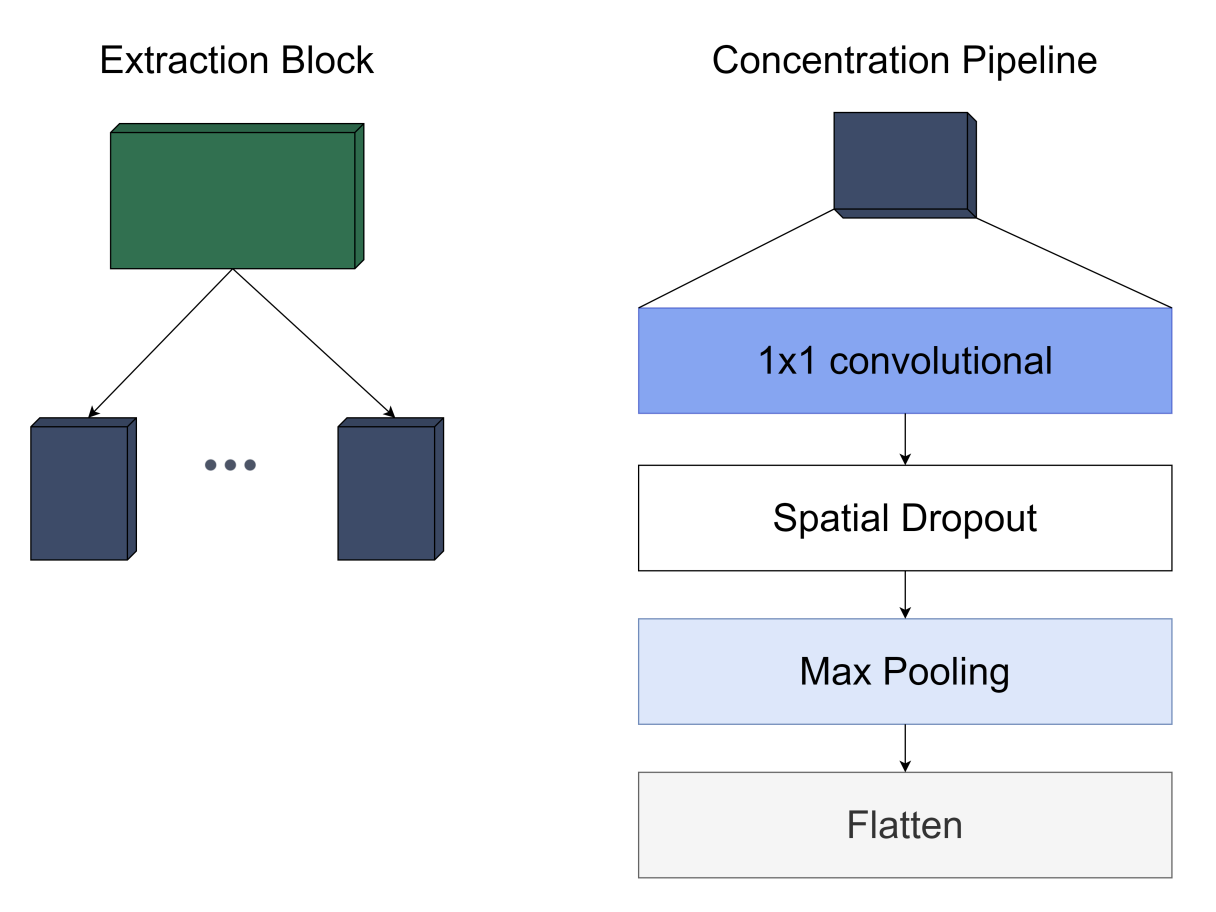
\includegraphics[width=\linewidth]{extraction.png}
        \caption{Extraction block.}
    \end{subfigure}
    \hfill
    \begin{subfigure}{0.48\textwidth}
        \centering
        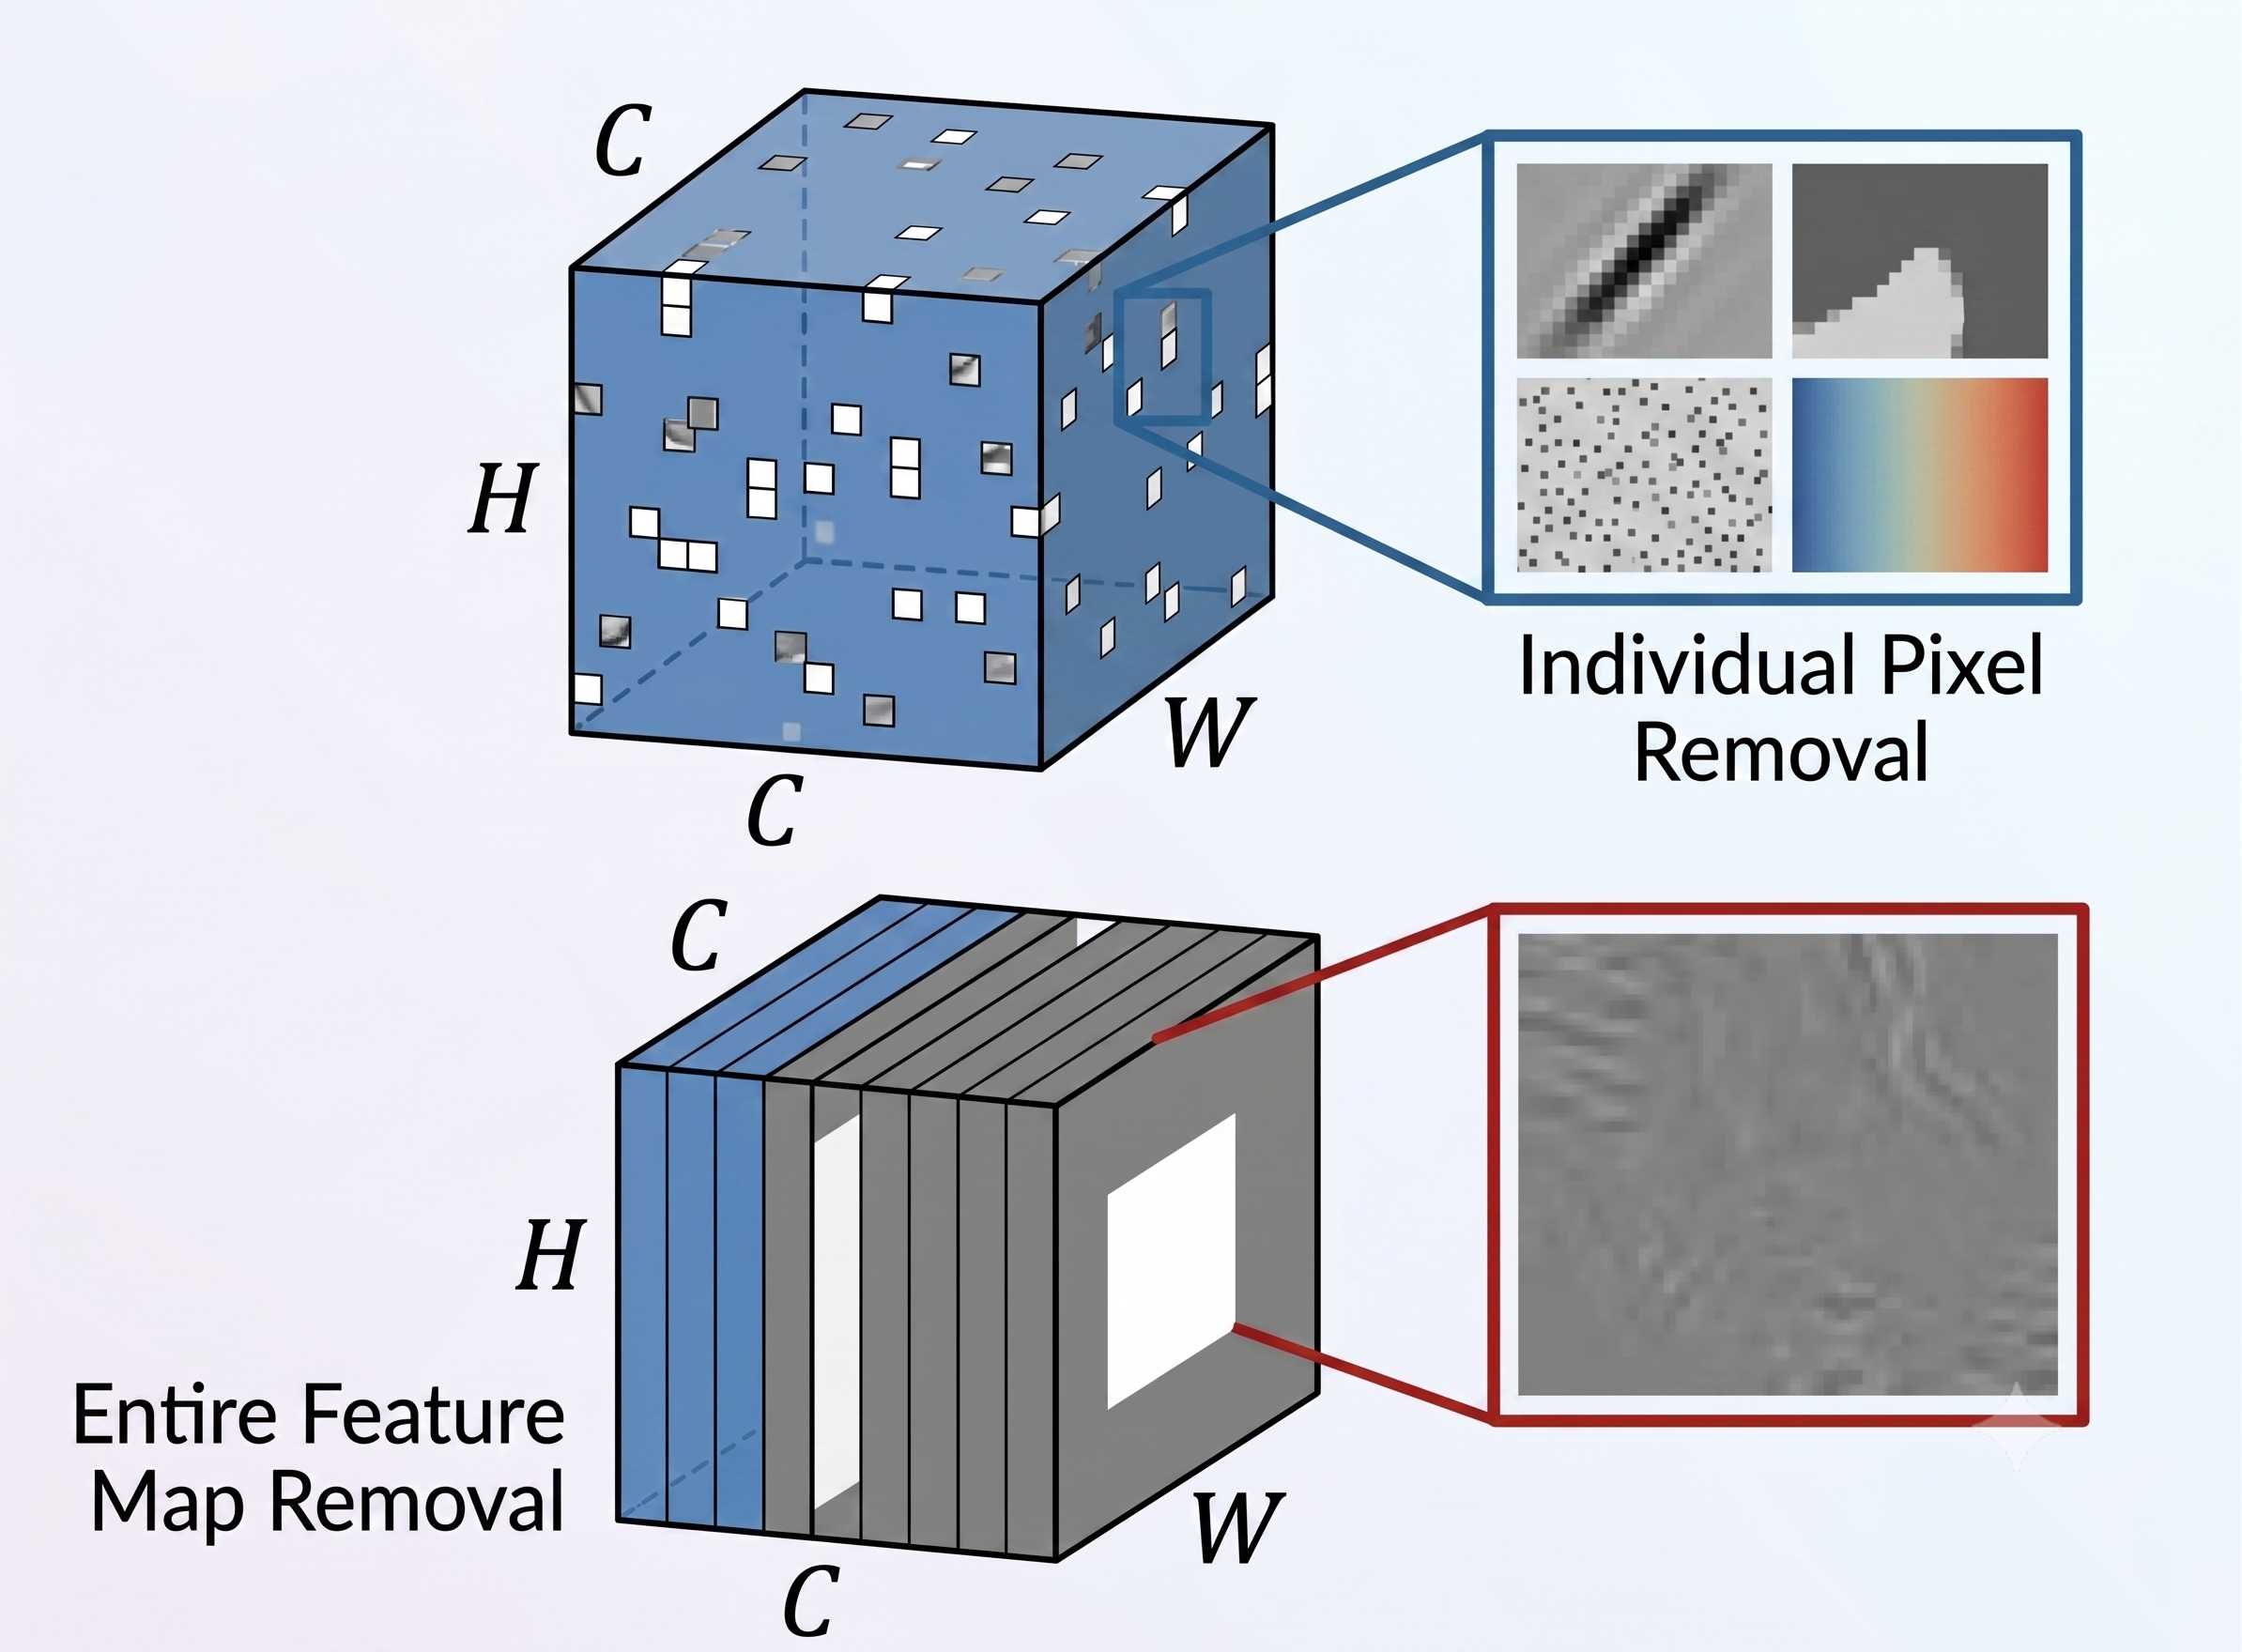
\includegraphics[width=\linewidth]{spatial_dropout.png}
        \caption{Spatial dropout intuition.}
    \end{subfigure}
    \caption{Core components used to transform intermediate convolutional features into compact multiscale representations.}
    \label{fig:extraction_block}
\end{figure}

\subsection{Contrastive Regularization}

The full \method{} model adds a supervised contrastive regularizer to the \base{} architecture. For a batch of $B$ samples, let $z_i^{(l)}$ be the normalized representation of sample $i$ extracted from layer $l$. For each anchor $i$, the positive set $\mathcal{P}(i)$ contains samples in the batch that share the same class label, while the negative set contains samples from other classes. A standard supervised contrastive objective can be written as
\[
    \mathcal{L}_{\mathrm{con}}^{(l)}
    =
    - \sum_{i=1}^{B}
    \frac{1}{|\mathcal{P}(i)|}
    \sum_{p \in \mathcal{P}(i)}
    \log
    \frac{
        \exp(\mathrm{sim}(z_i^{(l)}, z_p^{(l)})/\tau)
    }{
        \sum_{a \neq i}
        \exp(\mathrm{sim}(z_i^{(l)}, z_a^{(l)})/\tau)
    },
\]
where $\tau$ is the temperature and $\mathrm{sim}(\cdot,\cdot)$ is cosine similarity or an equivalent dot product over normalized vectors. The total training objective is
\[
    \mathcal{L}
    =
    \mathcal{L}_{\mathrm{CE}}
    +
    \alpha
    \sum_{l \in \mathcal{L}_{\mathrm{feat}}}
    \mathcal{L}_{\mathrm{con}}^{(l)} ,
\]
where $\mathcal{L}_{\mathrm{CE}}$ is cross-entropy and $\alpha$ controls the strength of the contrastive term. The default setting follows the paper: $\alpha=0.01$ and $\tau=1.0$.

\section{Implementation in the Project Codebase}

This section connects the method above to the submitted repository. It is included because a course project should make clear what has actually been implemented and how the experimental numbers are produced.

\subsection{Repository Organization}

The codebase is organized around a small number of modules. The most important files are summarized in Table~\ref{tab:codebase_map}.

\begin{table}[H]
\centering
\caption{Mapping from project files to their roles in the implementation.}
\label{tab:codebase_map}
\small
\begin{adjustbox}{max width=\textwidth}
\begin{tabular}{ll}
\toprule
File or folder & Role in the project \\
\midrule
\codepath{models/m2cl.py} & Builds ERM, \base{}, and \method{} ResNet-based architectures. \\
\codepath{models/extraction\_block.py} & Implements concentration pipelines, spatial dropout, pooling, and MLP projection. \\
\codepath{losses/contrastive.py} & Implements the layer-wise contrastive regularizer used by \method{}. \\
\codepath{algorithms/baselines.py} & Wraps M2/M2-CL and baseline algorithms behind a common training interface. \\
\codepath{tools/train.py} & Builds datasets, splits source domains, trains, validates, checkpoints, and writes metrics. \\
\codepath{data/} & Contains dataset loaders for PACS, VLCS, and Office-Home. \\
\codepath{configs/} & Stores default hyperparameters for each dataset. \\
\codepath{scripts/} & Provides shell scripts for full experiment grids and paper-style runs. \\
\codepath{reportcv/} & Contains this report, extracted paper text, and generated result tables. \\
\bottomrule
\end{tabular}
\end{adjustbox}
\end{table}

The implementation follows a useful separation of concerns. Model construction is separated from training logic, dataset loading is separated from experiment scripts, and the report tables are generated from result artifacts. This makes it possible to run small smoke tests, single-domain experiments, or complete paper-style grids without changing model code.

\subsection{Model Construction}

The local implementation defines three model families. \codepath{ERMResNet} keeps the standard ResNet classifier and returns logits plus an empty feature list. \codepath{OfficialM2} removes the final ResNet fully connected layer, registers forward hooks at selected intermediate layers, passes the captured activations through extraction blocks, concatenates the projected outputs, and classifies the resulting hypercolumn-like vector. \codepath{M2CL} is a backward-compatible name for the same architecture with returned intermediate energies enabled for contrastive learning.

For ResNet-18, the selected extraction points include 13 convolutional or residual outputs across \codepath{layer1} through \codepath{layer4}. For ResNet-50, the implementation attaches extraction blocks to bottleneck outputs and then selects a smaller subset for the final classifier. This design is consistent with the paper's motivation: ResNet-50 already has many more intermediate blocks, so concatenating every projected output would increase the classifier dimension and memory cost unnecessarily.

The project uses PyTorch forward hooks to collect intermediate tensors. This is a pragmatic implementation choice. It avoids rewriting the ResNet forward pass manually, while still allowing the extraction blocks to access activations inside the backbone. The tradeoff is that the model must carefully clear the temporary feature dictionary before each forward pass and remove hooks if the model object is no longer needed.

\subsection{Extraction Block Details}

The extraction block in \codepath{models/extraction\_block.py} has two supported modes: parallel and cascading. In the parallel mode, each pooling size has its own concentration pipeline. In the cascading mode, all pooling paths share the same compressed feature map. The default project configuration uses the parallel pipeline because the ablation table and the paper both indicate stronger overall performance.

Each concentration pipeline applies:

\begin{enumerate}[leftmargin=1.6em]
    \item a $1 \times 1$ convolution for channel compression,
    \item \codepath{Dropout2d} for spatial dropout,
    \item max pooling with a selected pool size,
    \item ReLU activation,
    \item flattening over the spatial grid, and
    \item an MLP projection from pooled spatial dimension to a compact vector.
\end{enumerate}

The MLP returns both the projected vector used by the classifier and an intermediate hidden activation called ``energy'' in the code. The classifier uses the projected vector, while the contrastive loss uses the energy activations. This small implementation detail is important because the contrastive term is not applied directly to the final logits. It regularizes intermediate representations before the final classification head.

\subsection{Loss Implementation}

The contrastive-loss module first computes cross-entropy on the final logits. If the method is \base{}, the contrastive weight is set to zero. If the method is \method{}, the loss subtracts a weighted layer score from cross-entropy:
\[
    \mathcal{L}_{\mathrm{impl}}
    =
    \mathcal{L}_{\mathrm{CE}}
    -
    \alpha \sum_l S_l .
\]
Here $S_l$ is larger when same-class pairs have high normalized similarity within layer $l$. Therefore, minimizing $\mathcal{L}_{\mathrm{impl}}$ encourages higher same-class similarity. In the code, activations are L2-normalized, pairwise similarities are exponentiated, positive same-class pairs are summed, and the score is compared against a full-batch denominator.

This implementation has a direct practical implication: the quality of the contrastive signal depends on the batch containing enough same-class pairs. With small batches or datasets with many classes, some classes may appear only once in a batch, giving little or no positive-pair signal for that class. This is one reason the default batch size is 128 when memory allows.

\subsection{Training Pipeline}

The training entry point loads dataset defaults from the configuration folder, then resolves command-line overrides. For PACS, VLCS, and Office-Home, \codepath{build\_datasets} constructs a leave-one-domain-out split: the chosen test domain becomes the unseen target, and the remaining domains become source environments.

The project also performs a DomainBed-style source validation split. Each source environment is split independently into train and validation subsets using a seeded hash. The default holdout fraction is 0.2. This is important because model selection should use source validation accuracy rather than target-domain test accuracy. Using target accuracy to choose checkpoints would violate the DG protocol.

During training, \codepath{M2Algorithm.update} concatenates minibatches across source environments, runs the model, computes the combined classification and contrastive objective, and updates the optimizer. The best checkpoint is selected by validation accuracy when a validation loader exists. After training, the best checkpoint is reloaded and evaluated on the held-out target domain. Metrics are saved as JSON files, which are later aggregated into result tables.

\subsection{Configuration Defaults}

The project uses paper-oriented defaults for \base{} and \method{}: ImageNet-pretrained ResNet-18 or ResNet-50, SGD optimizer, learning rate $0.001$, 30 epochs, batch size 128, reduction ratio $r=4$, dropout probability 0.3, contrastive weight $\alpha=0.01$, and temperature $\tau=1.0$. Baseline methods use separate defaults that are closer to DomainBed-style recommendations. This distinction is reasonable because M2/M2-CL and the comparison baselines have different optimization behavior.

\section{Reproduction Workflow}

The repository expects datasets to be placed under a common data root and provides \codepath{tools/check\_data.py} to validate folder layout before long runs. A single PACS run with \method{} can be launched as:
\[
    \texttt{\small python tools/train.py --dataset pacs --test\_domain photo --method m2cl}
\]
VLCS and Office-Home use the same pattern with different dataset and domain arguments.

For full paper-style experiments, \codepath{tools/run\_experiments.py} and the scripts under \codepath{scripts/} iterate over datasets, target domains, methods, backbones, and seeds. The intended score for each benchmark is the average over held-out target domains and random seeds. The training script saves the checkpoint with the best source validation accuracy, reloads it after training, evaluates the held-out target domain, and writes metric JSON files for later aggregation.

\section{Experimental Setup}

\subsection{Datasets}

The project uses three DG benchmarks:

\begin{itemize}
    \item \textbf{PACS}: 9,991 images, 7 classes, and 4 domains: Photo, Art Painting, Cartoon, and Sketch.
    \item \textbf{VLCS}: 10,729 images, 5 classes, and 4 domains: PASCAL VOC, LabelMe, Caltech101, and SUN09.
    \item \textbf{Office-Home}: 15,588 images, 65 classes, and 4 domains: Art, Clipart, Product, and Real-World.
\end{itemize}

For each dataset, the evaluation follows the leave-one-domain-out protocol. One domain is used as the target test domain, and the remaining domains are used for training and validation. The reported metric is top-1 classification accuracy on the held-out target domain.

\begin{figure}[H]
    \centering
    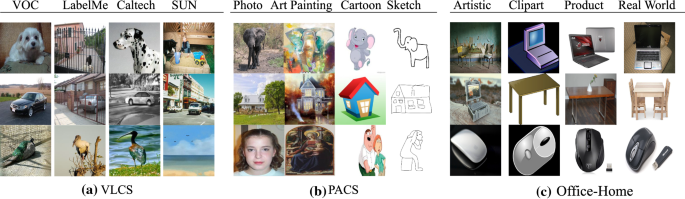
\includegraphics[width=0.72\textwidth]{dataset_cv1.png}
    \caption{Datasets used in the slide deck and project experiments: PACS, VLCS, and Office-Home.}
    \label{fig:datasets}
\end{figure}

\subsection{Training Configuration}

The training setting follows the paper-oriented configuration used in the project:

\begin{itemize}
    \item Backbones: ResNet-18 and ResNet-50 pretrained on ImageNet.
    \item Optimizer: stochastic gradient descent.
    \item Training length: 30 epochs for each domain split.
    \item Learning rate: 0.001.
    \item Batch size: 128 when GPU memory allows.
    \item Extraction reduction factor: $r=4$.
    \item Contrastive loss weight: $\alpha=0.01$.
    \item Temperature: $\tau=1.0$.
\end{itemize}

\subsection{Baselines}

The reported comparison includes ERM, RSC, CORAL, Mixup, MMD, SagNet, SelfReg, ARM, EQRM, and SAGM. These methods cover a broad range of DG strategies: standard supervised learning, representation suppression, feature distribution alignment, sample interpolation, style robustness, self-supervised regularization, adaptive risk learning, and sharpness-aware generalization.

\section{Quantitative Results}

Table~\ref{tab:summary_results} summarizes the main benchmark averages presented in the slides. The full per-domain tables are included in the appendix.

\begin{table}[H]
\centering
\caption{Main average top-1 accuracy and gains over the best baseline. Higher is better.}
\label{tab:summary_results}
\small
\begin{adjustbox}{max width=\textwidth}
\begin{tabular}{llrrrrrr}
\toprule
\rowcolor{headerblue}
Backbone & Method & PACS & $\Delta$ & VLCS & $\Delta$ & Office-Home & $\Delta$ \\
\midrule
ResNet-18 & Best baseline & 81.07 & -- & 77.57 & -- & 63.35 & -- \\
ResNet-18 & \base{} & 81.81 & \pos{0.74} & 78.00 & \pos{0.43} & 63.47 & \pos{0.12} \\
\rowcolor{lightgreen}
ResNet-18 & \textbf{\method{}} & \textbf{82.51} & \textbf{\pos{1.44}} & \textbf{78.50} & \textbf{\pos{0.93}} & \textbf{64.18} & \textbf{\pos{0.83}} \\
\midrule
ResNet-50 & Best baseline & 84.89 & -- & 78.10 & -- & 67.33 & -- \\
ResNet-50 & \base{} & 86.11 & \pos{1.22} & 78.76 & \pos{0.66} & 68.70 & \pos{1.37} \\
\rowcolor{lightgreen}
ResNet-50 & \textbf{\method{}} & \textbf{86.56} & \textbf{\pos{1.67}} & \textbf{79.09} & \textbf{\pos{0.99}} & \textbf{69.34} & \textbf{\pos{2.01}} \\
\bottomrule
\end{tabular}
\end{adjustbox}
\end{table}

The improved table makes the trend easier to read. \base{} already beats the strongest baseline in every summarized setting, so the multiscale architecture itself is useful. \method{} then improves over both the best baseline and \base{}, showing that the contrastive regularizer adds a second source of gain. The largest improvement appears on Office-Home with ResNet-50 (\pos{2.01}), which suggests that the stronger backbone benefits more from the additional intermediate representations.

\begin{table}[H]
\centering
\caption{Compact interpretation of the experimental results.}
\label{tab:result_interpretation}
\small
\begin{adjustbox}{max width=\textwidth}
\begin{tabular}{llll}
\toprule
\rowcolor{headerblue}
Comparison & ResNet-18 Avg Gain & ResNet-50 Avg Gain & Interpretation \\
\midrule
\base{} vs. best baseline & \pos{0.43} & \pos{1.08} & Multilayer/multiscale features help even without contrastive loss. \\
\method{} vs. best baseline & \textbf{\pos{1.07}} & \textbf{\pos{1.56}} & Full method gives consistent average improvement. \\
\method{} vs. \base{} & \pos{0.64} & \pos{0.47} & Contrastive loss gives a smaller but stable extra gain. \\
\bottomrule
\end{tabular}
\end{adjustbox}
\end{table}

The results show a consistent trend across backbones and datasets. This supports the paper's central claim that intermediate multiscale features are useful for DG, and that explicitly aligning same-class representations across source domains can improve robustness.

The improvement is not uniform across every individual target domain. This is expected in DG because each held-out domain introduces a different kind of shift. Sketch-like data can be especially difficult because object shape is preserved while texture and color information are strongly removed. Office-Home is also challenging because it contains many more classes than PACS and VLCS, making class-level alignment harder.

\subsection{Per-Dataset Interpretation}

PACS is the most intuitive dataset for DG because the domain shift is visible: photo, art painting, cartoon, and sketch images share object categories but differ strongly in texture and style. Improvements on PACS suggest that the model is not only memorizing domain-specific appearance. The saliency examples also support this interpretation because \method{} tends to focus more on object contours and parts.

VLCS is less stylized than PACS but combines images from different dataset sources. Here the domain shift is often caused by collection bias, background, object scale, and scene composition. The gains are usually smaller than in PACS, which is reasonable because the visual shift is subtler and the class set is smaller.

Office-Home is more difficult because it contains 65 classes. The larger number of classes makes the contrastive term harder to optimize: a batch of 128 may still contain few positive pairs for some classes, especially if source-domain sampling is imbalanced. Improvements on Office-Home are therefore meaningful, but they also depend strongly on batch composition and full multi-seed evaluation.

\begin{table}[H]
\centering
\caption{Dataset-level reading of the experimental results.}
\label{tab:dataset_reading}
\small
\begin{adjustbox}{max width=\textwidth}
\begin{tabular}{llll}
\toprule
\rowcolor{headerblue}
Dataset & Main shift type & Observed behavior & Practical comment \\
\midrule
PACS & Style and texture shift & \method{} improves over baseline on both backbones. & Good benchmark for showing sketch/cartoon robustness. \\
VLCS & Dataset-source bias & Gain is positive but smaller than PACS. & Shift is subtler; improvements should be checked over seeds. \\
Office-Home & Many classes and style variation & Strongest ResNet-50 gain appears here. & Batch composition matters because positive pairs are sparser. \\
\bottomrule
\end{tabular}
\end{adjustbox}
\end{table}

\subsection{What the Numbers Suggest About the Method}

The average results support two separate claims. First, the \base{} architecture usually improves over the best baseline, suggesting that multilayer and multiscale features are useful even without contrastive regularization. Second, \method{} improves over \base{}, suggesting that the contrastive term adds value beyond architecture alone.

However, the magnitude of improvement should be interpreted carefully. A difference of less than one percentage point may be meaningful only if averaged over enough seeds. DG benchmarks are sensitive to random initialization, validation split, data augmentation, and target-domain choice. Therefore, the best use of the current report is to understand the mechanism and the implementation; the final leaderboard-style claim should wait for complete real runs.

\section{Ablation and Sensitivity Analysis}

The ablation study isolates the effect of four design choices: the extraction pipeline type, the reduction factor $r$, spatial dropout, and the additional contrastive loss. The strongest configuration in the project slides is the parallel pipeline with $r=4$, spatial dropout, and contrastive loss. Compared with the same setting without the contrastive objective, the full configuration improves PACS average from 79.15 to 80.10 and VLCS average from 73.14 to 74.15.

The sensitivity study evaluates the effect of $\tau$ and $\alpha$. Temperature changes the concentration of the contrastive distribution. A very small or very large temperature can make the contrastive signal unstable or insufficiently discriminative. The loss weight $\alpha$ is also important: when it is too large, the contrastive objective can dominate cross-entropy and hurt classification. In the slide results, $\alpha=10^{-1}$ produces a large degradation, which is consistent with the intuition that the contrastive term should regularize the classifier rather than replace the supervised objective.

\begin{table}[H]
\centering
\caption{Interpretation of the ablation and sensitivity study.}
\label{tab:ablation_interpretation}
\small
\begin{adjustbox}{max width=\textwidth}
\begin{tabular}{llll}
\toprule
\rowcolor{headerblue}
Design choice & Tested variants & Best project setting & Interpretation \\
\midrule
Pipeline layout & cascading, parallel & parallel & Separate scale-specific pipelines preserve richer evidence. \\
Reduction ratio $r$ & 2, 4, 6 & 4 & Balances compactness and information retention. \\
Dropout type & with/without spatial dropout & with dropout & Reduces dependence on correlated feature maps. \\
Contrastive weight $\alpha$ & $0$ to $10^{-1}$ & small nonzero value & Helpful as regularizer; harmful when too dominant. \\
Temperature $\tau$ & small to very large values & around paper default & Controls sharpness of pair similarity distribution. \\
\bottomrule
\end{tabular}
\end{adjustbox}
\end{table}

\subsection{Design Lessons from the Ablation}

The ablation results are useful because they separate the architecture into decisions that can be reasoned about independently. The first decision is whether concentration pipelines should be cascading or parallel. Cascading pipelines reuse the same compressed map, which saves parameters, but each scale receives information after the same channel bottleneck. Parallel pipelines allow each scale to learn its own compression before pooling, which is more flexible. The project uses the parallel setting because the average results are stronger.

The second decision is the reduction ratio $r$. A small $r$ keeps more channels and therefore preserves more information, but it increases memory and may pass too much domain-specific detail to the classifier. A large $r$ reduces memory, but it can remove useful class evidence. The selected value $r=4$ is a compromise between representation capacity and regularization.

The third decision is spatial dropout. In convolutional feature maps, neighboring activations are correlated. Standard dropout can remove isolated values while leaving adjacent evidence nearly unchanged. Spatial dropout removes whole channels, making the model less dependent on any single feature map. In a DG setting, this is a useful inductive bias because shortcuts often appear as repeated feature channels associated with texture or background.

The fourth decision is the contrastive loss itself. The ablation indicates that contrastive learning is helpful when it is used as a weak regularizer. This matches the implementation: the main task is still classification by cross-entropy, while the contrastive term shapes intermediate representations. When $\alpha$ is too large, the representation objective can overpower class prediction and degrade accuracy.

\section{Qualitative Results}

The qualitative analysis uses saliency maps to visualize which pixels contribute most strongly to the model's prediction. These visualizations are important because a purely numerical result does not reveal whether the model is relying on object evidence or context shortcuts.

\begin{figure}[H]
    \centering
    
\includegraphics[width=0.78\textwidth]{Pacs.png}
    \caption{PACS saliency maps comparing a baseline model and \method{}. Darker regions indicate pixels with stronger influence on the predicted class.}
    \label{fig:saliency}
\end{figure}

The saliency maps indicate that ERM can assign strong importance to background and domain-specific context. In contrast, \method{} tends to concentrate more on object regions and object boundaries. This behavior is aligned with the quantitative results: a model that ignores unstable background cues is more likely to generalize when the target domain changes.

\begin{figure}[H]
    \centering
    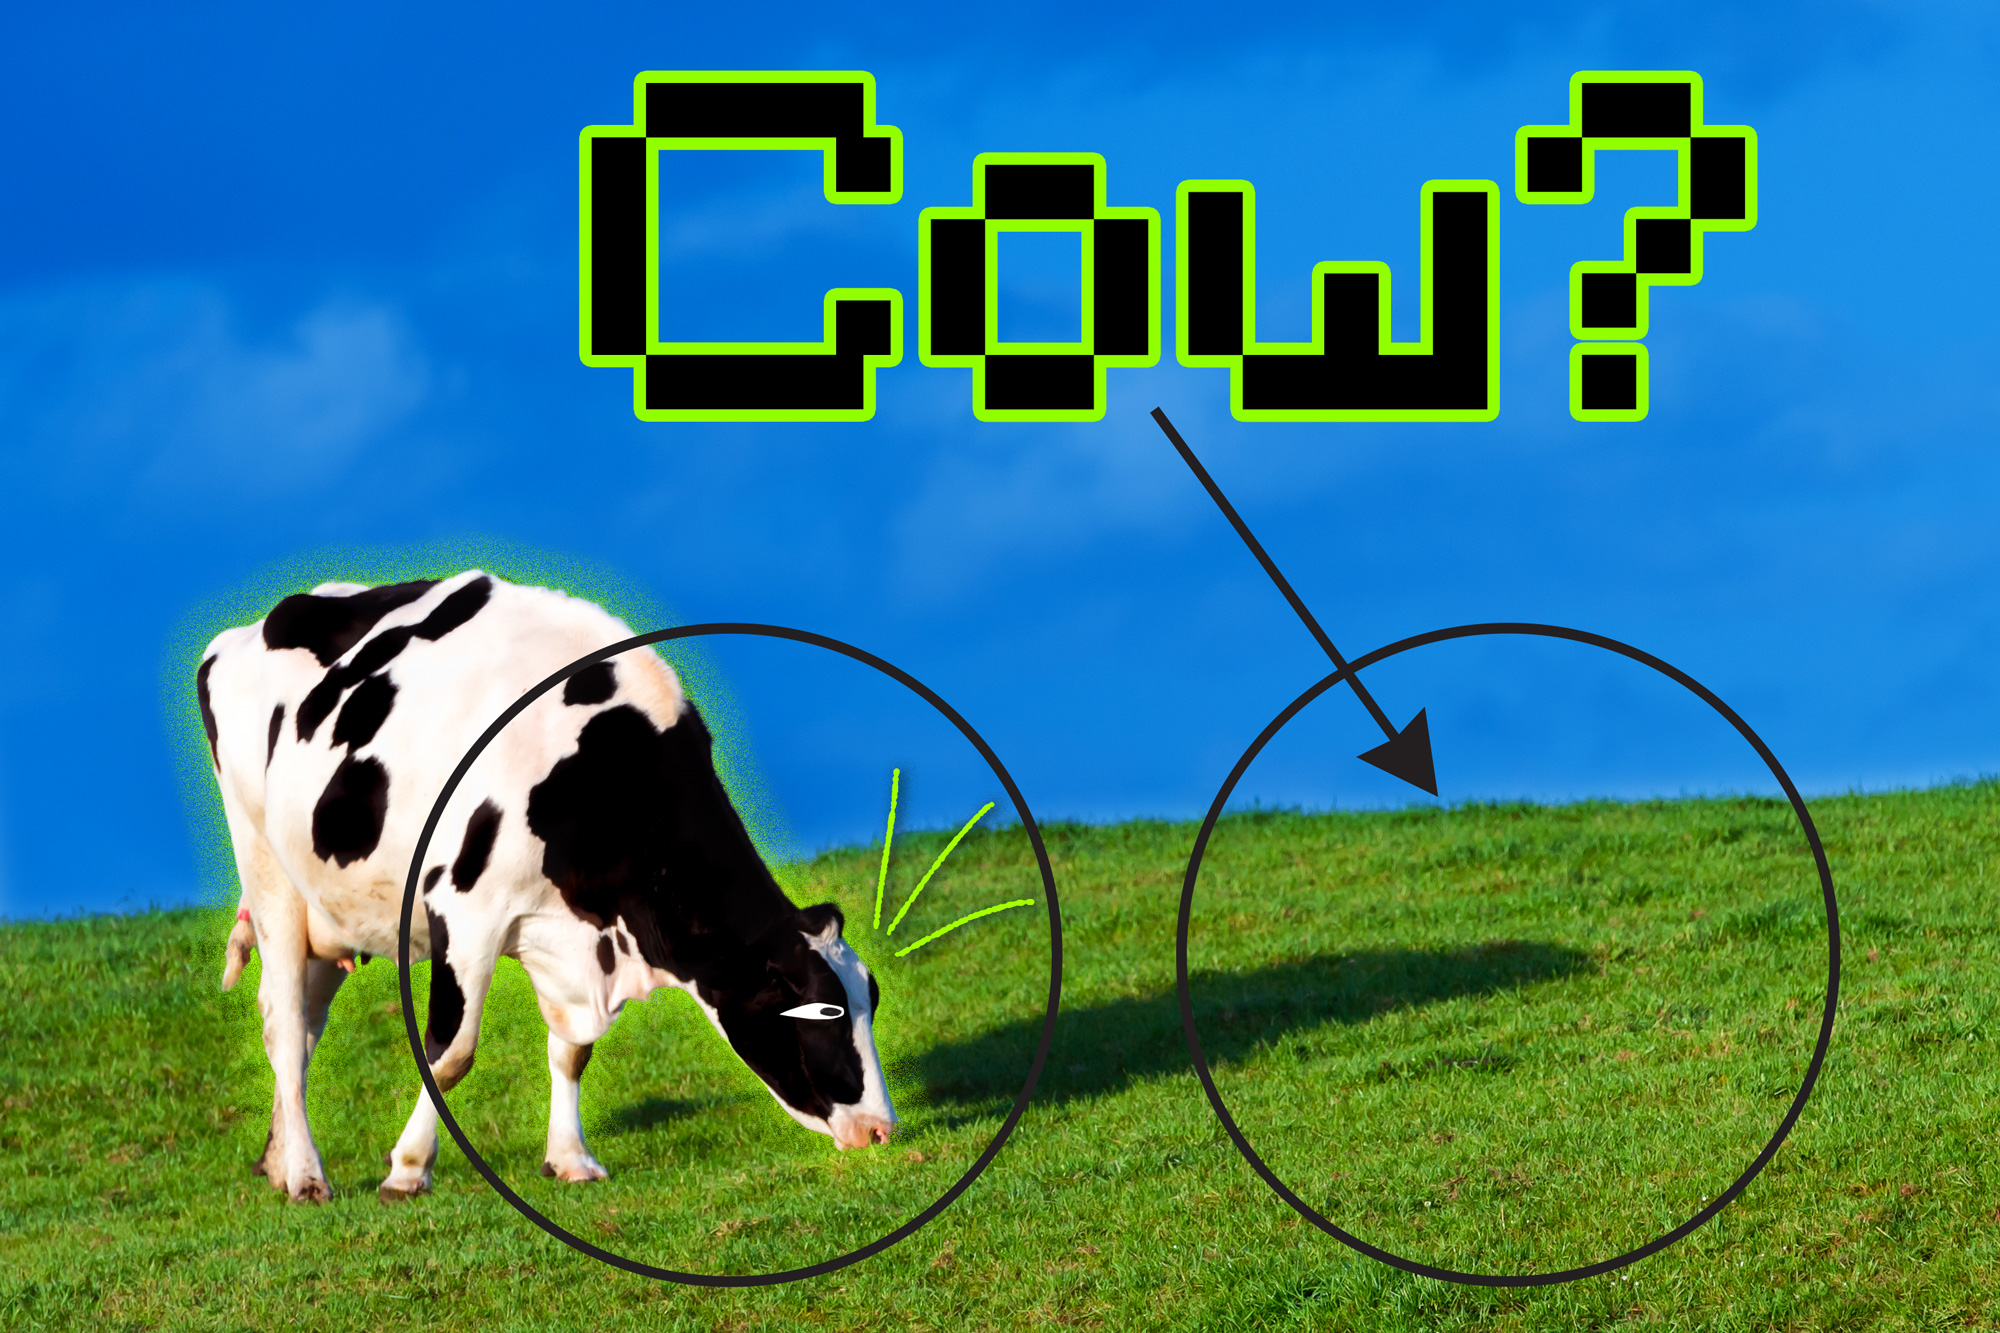
\includegraphics[width=0.72\textwidth]{failure_1.jpg}
    \caption{Example image used as a qualitative failure-case reminder. Complex backgrounds and unusual context can still confuse a model if class and context cues are strongly entangled.}
    \label{fig:failure_case}
\end{figure}

\subsection{How to Read the Saliency Maps}

The qualitative figures should not be interpreted as a formal proof of causality. Saliency maps are sensitive to gradient saturation, preprocessing, and model confidence. Their value in this report is diagnostic: they provide a visual sanity check for the shortcut-learning hypothesis. If ERM highlights the background while \method{} highlights object parts, then the visualization is consistent with the claim that multilayer contrastive regularization changes the model's attention pattern.

The examples are also helpful for explaining DG to a non-specialist reader. A classifier that predicts ``dog'' because of grass or ``guitar'' because of a studio-like background may work on the source data but fail in a new domain. A classifier that relies more on object shape, boundary, and parts has a better chance of transferring to sketches, cartoons, or different camera conditions.

Figure~\ref{fig:failure_case} is included to keep the qualitative discussion realistic. \method{} reduces shortcut reliance, but it does not guarantee perfect causal recognition. When the object is small, occluded, or surrounded by a visually dominant context, intermediate features can still contain mixed class and domain evidence. This is why the report treats saliency maps as supporting evidence rather than final proof.

\section{Discussion}

The project results support three main conclusions. First, using intermediate representations is beneficial because it gives the classifier access to visual evidence at several semantic depths. Early layers preserve local textures and edges, middle layers capture object parts, and deeper layers encode more abstract class-related concepts. Combining them gives the model a richer representation than using only the final ResNet feature.

Second, spatial dropout is useful because it regularizes whole feature maps rather than isolated pixels. Since convolutional activations are spatially correlated, ordinary dropout may leave enough neighboring information for a shortcut to survive. Dropping entire maps makes the extraction block less dependent on narrow local patterns.

Third, the contrastive loss improves class-level compactness. By pulling together same-class representations and pushing apart different classes, \method{} encourages domain-invariant clustering in latent space. However, the sensitivity analysis shows that this term must be carefully weighted. A contrastive loss that is too strong can interfere with cross-entropy optimization.

\subsection{Comparison with the Original Paper}

The original paper is written for a research audience and prioritizes novelty, state-of-the-art comparisons, and compact mathematical presentation. This report has a different purpose. It explains how the method is reconstructed in code and how the training protocol is organized for a course project. Several differences should be noted:

\begin{itemize}[leftmargin=1.4em]
    \item The original paper includes broader benchmark coverage, while this project report focuses quantitatively on PACS, VLCS, and Office-Home.
    \item The paper presents final benchmark tables. This report reorganizes the project-table results around the defense narrative and implementation details.
    \item The paper describes the architecture abstractly. This report maps the architecture to PyTorch modules, forward hooks, extraction blocks, and training scripts.
    \item The paper emphasizes the method's accuracy. This report also emphasizes reproducibility, code organization, and limitations of the current experiment set.
\end{itemize}

These differences make the document more suitable for a university submission. The goal is not to claim a new research contribution, but to demonstrate understanding, implementation ability, and critical evaluation.

\subsection{Practical Engineering Observations}

Implementing \method{} is more involved than implementing ERM. ERM only needs a backbone, a classifier, and cross-entropy. In contrast, \method{} requires collecting intermediate activations, maintaining extraction blocks for different layer shapes, concatenating many projected vectors, and computing a layer-wise pair objective. This increases the number of moving parts and makes debugging more important.

The forward-hook design is concise, but it also creates hidden state inside the model. The feature dictionary must be cleared at the beginning of each forward pass. If hooks are accidentally duplicated, the model can store unexpected activations or waste memory. The current implementation handles this by registering hooks during initialization and exposing a \codepath{remove\_hooks} method.

Memory is another practical issue. Extraction blocks create additional tensors before and after pooling, and the contrastive loss computes batch-level pairwise similarities. Larger backbones, larger batches, and more extraction points all increase GPU memory demand. This explains why the batch size and selected ResNet-50 outputs are important design choices rather than arbitrary details.

\subsection{Threats to Validity}

There are three main threats to validity in the current project. First, incomplete or partially repeated runs limit the strength of quantitative conclusions. Second, single-run trends may not represent the true average because DG performance can vary across random seeds. Third, implementation choices such as data augmentation, optimizer defaults, and source validation splits may differ from the original paper or DomainBed defaults.

Despite these threats, the project remains valuable because the architecture, loss, and training protocol are implemented in a transparent way. The report also identifies exactly which parts need more computation before the reproduction can be considered complete.

\section{Course Project Reflection}

The main lesson from the project is that DG is a representation-learning problem, not only a benchmark protocol. A model can achieve high source accuracy while learning features that are unstable outside the training domains. \method{} addresses this by combining intermediate CNN evidence with a contrastive term that encourages same-class consistency across domains.

The second lesson is about reproducibility. A convincing DG experiment requires careful source-target separation, source-only checkpoint selection, multiple seeds, and clear result aggregation. The most important future improvement is therefore completing additional repeated runs, then reporting both mean and standard deviation. Additional useful extensions include memory/time profiling and failure-case saliency analysis.

\section{Limitations}

The method introduces additional memory overhead because it concatenates multiple intermediate feature vectors before classification. This is particularly relevant for ResNet-50 and for large batch sizes. The contrastive component also depends on batch composition: if a batch contains too few positive pairs per class, the contrastive signal becomes weaker.

\section{Conclusion}

This report presented a detailed study of \method{} for domain generalization. The method addresses shortcut learning by extracting multiscale representations from intermediate CNN layers and by applying a supervised contrastive loss to improve class-level alignment across source domains. On PACS, VLCS, and Office-Home, the summarized results show that \method{} improves average accuracy over strong DG baselines under both ResNet-18 and ResNet-50 backbones. Qualitative saliency maps further suggest that the method focuses more on object-relevant regions and less on unstable context. Overall, the project demonstrates that multilayer feature reuse and carefully weighted contrastive regularization are effective tools for improving robustness to unseen visual domains.

\appendix
\section{Full Result Tables}

The following pages reproduce the full result tables used in the slide deck.

\begin{figure}[H]
    \centering
    
\includegraphics[page=1,width=\textwidth]{result_tables.pdf}
    \caption{Full result tables, page 1.}
\end{figure}

\begin{figure}[H]
    \centering
    
\includegraphics[page=2,width=\textwidth]{result_tables.pdf}
    \caption{Full result tables, page 2.}
\end{figure}

\section{References}

\begin{thebibliography}{9}

\bibitem{ballas2024m2cl}
A. Ballas and C. Diou,
\textit{Multiscale and Multilayer Contrastive Learning for Domain Generalization},
IEEE Transactions on Artificial Intelligence, 2024.

\bibitem{domainbed}
I. Gulrajani and D. Lopez-Paz,
\textit{In Search of Lost Domain Generalization},
International Conference on Learning Representations, 2021.

\bibitem{resnet}
K. He, X. Zhang, S. Ren, and J. Sun,
\textit{Deep Residual Learning for Image Recognition},
IEEE Conference on Computer Vision and Pattern Recognition, 2016.

\bibitem{pacs}
D. Li, Y. Yang, Y.-Z. Song, and T. M. Hospedales,
\textit{Deeper, Broader and Artier Domain Generalization},
IEEE International Conference on Computer Vision, 2017.

\bibitem{officehome}
H. Venkateswara, J. Eusebio, S. Chakraborty, and S. Panchanathan,
\textit{Deep Hashing Network for Unsupervised Domain Adaptation},
IEEE Conference on Computer Vision and Pattern Recognition, 2017.

\end{thebibliography}

\end{document}
